% Options for packages loaded elsewhere
\PassOptionsToPackage{unicode}{hyperref}
\PassOptionsToPackage{hyphens}{url}
%
\documentclass[
]{article}
\usepackage{amsmath,amssymb}
\usepackage{lmodern}
\usepackage{iftex}
\ifPDFTeX
  \usepackage[T1]{fontenc}
  \usepackage[utf8]{inputenc}
  \usepackage{textcomp} % provide euro and other symbols
\else % if luatex or xetex
  \usepackage{unicode-math}
  \defaultfontfeatures{Scale=MatchLowercase}
  \defaultfontfeatures[\rmfamily]{Ligatures=TeX,Scale=1}
\fi
% Use upquote if available, for straight quotes in verbatim environments
\IfFileExists{upquote.sty}{\usepackage{upquote}}{}
\IfFileExists{microtype.sty}{% use microtype if available
  \usepackage[]{microtype}
  \UseMicrotypeSet[protrusion]{basicmath} % disable protrusion for tt fonts
}{}
\makeatletter
\@ifundefined{KOMAClassName}{% if non-KOMA class
  \IfFileExists{parskip.sty}{%
    \usepackage{parskip}
  }{% else
    \setlength{\parindent}{0pt}
    \setlength{\parskip}{6pt plus 2pt minus 1pt}}
}{% if KOMA class
  \KOMAoptions{parskip=half}}
\makeatother
\usepackage{xcolor}
\usepackage[margin=1in]{geometry}
\usepackage{color}
\usepackage{fancyvrb}
\newcommand{\VerbBar}{|}
\newcommand{\VERB}{\Verb[commandchars=\\\{\}]}
\DefineVerbatimEnvironment{Highlighting}{Verbatim}{commandchars=\\\{\}}
% Add ',fontsize=\small' for more characters per line
\usepackage{framed}
\definecolor{shadecolor}{RGB}{248,248,248}
\newenvironment{Shaded}{\begin{snugshade}}{\end{snugshade}}
\newcommand{\AlertTok}[1]{\textcolor[rgb]{0.94,0.16,0.16}{#1}}
\newcommand{\AnnotationTok}[1]{\textcolor[rgb]{0.56,0.35,0.01}{\textbf{\textit{#1}}}}
\newcommand{\AttributeTok}[1]{\textcolor[rgb]{0.77,0.63,0.00}{#1}}
\newcommand{\BaseNTok}[1]{\textcolor[rgb]{0.00,0.00,0.81}{#1}}
\newcommand{\BuiltInTok}[1]{#1}
\newcommand{\CharTok}[1]{\textcolor[rgb]{0.31,0.60,0.02}{#1}}
\newcommand{\CommentTok}[1]{\textcolor[rgb]{0.56,0.35,0.01}{\textit{#1}}}
\newcommand{\CommentVarTok}[1]{\textcolor[rgb]{0.56,0.35,0.01}{\textbf{\textit{#1}}}}
\newcommand{\ConstantTok}[1]{\textcolor[rgb]{0.00,0.00,0.00}{#1}}
\newcommand{\ControlFlowTok}[1]{\textcolor[rgb]{0.13,0.29,0.53}{\textbf{#1}}}
\newcommand{\DataTypeTok}[1]{\textcolor[rgb]{0.13,0.29,0.53}{#1}}
\newcommand{\DecValTok}[1]{\textcolor[rgb]{0.00,0.00,0.81}{#1}}
\newcommand{\DocumentationTok}[1]{\textcolor[rgb]{0.56,0.35,0.01}{\textbf{\textit{#1}}}}
\newcommand{\ErrorTok}[1]{\textcolor[rgb]{0.64,0.00,0.00}{\textbf{#1}}}
\newcommand{\ExtensionTok}[1]{#1}
\newcommand{\FloatTok}[1]{\textcolor[rgb]{0.00,0.00,0.81}{#1}}
\newcommand{\FunctionTok}[1]{\textcolor[rgb]{0.00,0.00,0.00}{#1}}
\newcommand{\ImportTok}[1]{#1}
\newcommand{\InformationTok}[1]{\textcolor[rgb]{0.56,0.35,0.01}{\textbf{\textit{#1}}}}
\newcommand{\KeywordTok}[1]{\textcolor[rgb]{0.13,0.29,0.53}{\textbf{#1}}}
\newcommand{\NormalTok}[1]{#1}
\newcommand{\OperatorTok}[1]{\textcolor[rgb]{0.81,0.36,0.00}{\textbf{#1}}}
\newcommand{\OtherTok}[1]{\textcolor[rgb]{0.56,0.35,0.01}{#1}}
\newcommand{\PreprocessorTok}[1]{\textcolor[rgb]{0.56,0.35,0.01}{\textit{#1}}}
\newcommand{\RegionMarkerTok}[1]{#1}
\newcommand{\SpecialCharTok}[1]{\textcolor[rgb]{0.00,0.00,0.00}{#1}}
\newcommand{\SpecialStringTok}[1]{\textcolor[rgb]{0.31,0.60,0.02}{#1}}
\newcommand{\StringTok}[1]{\textcolor[rgb]{0.31,0.60,0.02}{#1}}
\newcommand{\VariableTok}[1]{\textcolor[rgb]{0.00,0.00,0.00}{#1}}
\newcommand{\VerbatimStringTok}[1]{\textcolor[rgb]{0.31,0.60,0.02}{#1}}
\newcommand{\WarningTok}[1]{\textcolor[rgb]{0.56,0.35,0.01}{\textbf{\textit{#1}}}}
\usepackage{graphicx}
\makeatletter
\def\maxwidth{\ifdim\Gin@nat@width>\linewidth\linewidth\else\Gin@nat@width\fi}
\def\maxheight{\ifdim\Gin@nat@height>\textheight\textheight\else\Gin@nat@height\fi}
\makeatother
% Scale images if necessary, so that they will not overflow the page
% margins by default, and it is still possible to overwrite the defaults
% using explicit options in \includegraphics[width, height, ...]{}
\setkeys{Gin}{width=\maxwidth,height=\maxheight,keepaspectratio}
% Set default figure placement to htbp
\makeatletter
\def\fps@figure{htbp}
\makeatother
\setlength{\emergencystretch}{3em} % prevent overfull lines
\providecommand{\tightlist}{%
  \setlength{\itemsep}{0pt}\setlength{\parskip}{0pt}}
\setcounter{secnumdepth}{-\maxdimen} % remove section numbering
\usepackage{titling}
\pretitle{\begin{center}\LARGE\includegraphics[width=14cm]{HMS_DBMI_Logo.jpg}\\[\bigskipamount]}
\posttitle{\end{center}}
\ifLuaTeX
  \usepackage{selnolig}  % disable illegal ligatures
\fi
\IfFileExists{bookmark.sty}{\usepackage{bookmark}}{\usepackage{hyperref}}
\IfFileExists{xurl.sty}{\usepackage{xurl}}{} % add URL line breaks if available
\urlstyle{same} % disable monospaced font for URLs
\hypersetup{
  pdftitle={Identification of Prognostic Pathogenic Genes and Clinical Trends in Individuals with Glioblastoma},
  pdfauthor={Author: Kevin Liu},
  hidelinks,
  pdfcreator={LaTeX via pandoc}}

\title{Identification of Prognostic Pathogenic Genes and Clinical Trends
in Individuals with Glioblastoma}
\author{Author: Kevin Liu}
\date{2022-10-20}

\begin{document}
\maketitle

{
\setcounter{tocdepth}{2}
\tableofcontents
}
\newpage

\hypertarget{background}{%
\section{Background}\label{background}}

Glioblastoma (GBM) is a common cancer of the central nervous system and
affected individuals has shown poor prognosis despite the currently
available treatment options. {[}1{]} Furthermore, immune-related genes
have been shown to play a prominent role in tumor gene expression.
{[}1{]} Previously, Liang et al.~identified 24 immune genes related to
the prognosis of GBM using genes from the ImmPort database; of which,
the CCL1, LPA, and SH2D1B genes were identified as prognostic pathogenic
genes of GBM based on their calculated hazard ratios. {[}1-2{]}
Additionally, it was found that CCL1 is expressed at higher levels in
males relative to females while BMP1 and OSMR are expressed at higher
levels in those with ages greater than 50 years old. {[}1{]}

In this analysis, we hypothesize that the differential gene expression
of prognostic pathogenic genes between normal tissue samples and tumor
tissue samples will be the main driving factor influencing our principal
components (PCs). Therefore, this analysis aims to identify the
prognostic pathogenic genes using PCA, examine the gene expression
patterns and interrelationships of both samples from normal tissue and
GBM tissue via hierarchical clustering, and replicate the clinical
findings of differential gene expression based on age group and sex by
Liang et al.

Since the authors' analyses were based on the TCGA-GBM dataset, which is
readily available to the public, we will attempt to explore the utility
of PCA weights in the screening of prognostic pathogenic genes among the
24 immune genes in GBM instead of the usage of a hazard ratio. The usage
of PCA is justified here as we would anticipate that genes with the
highest relevance to the etiology of GBM to demonstrate the highest
relevance to the PCs that explain the most variance in our RNA-seq read
count data between each of the individuals.

Subsequently, we will attempt utilize hierarchical clustering to explore
the 24 immune gene expression patterns in terms of how each of the genes
are related to one another and whether sample subtypes can be clustered
based on the normalized RNA-seq read counts of the 24 immune genes for
each sample donor.

Finally, we will attempt to replicate the clinical findings between
select genes of interest and their associations with age group and sex
identified by Liang et al.

\hypertarget{references}{%
\subsection{References}\label{references}}

{[}1{]} Liang P, Chai Y, Zhao H, Wang G. Predictive Analyses of
Prognostic-Related Immune Genes and Immune Infiltrates for Glioblastoma.
Diagnostics (Basel). 2020;10(3):177. Published 2020 Mar 24.
\url{doi:10.3390/diagnostics10030177}

{[}2{]} Bhattacharya S, Dunn P, Thomas CG, et al.~ImmPort, toward
repurposing of open access immunological assay data for translational
and clinical research. Sci Data. 2018;5:180015. Published 2018 Feb 27.
\url{doi:10.1038/sdata.2018.15}

\newpage

\hypertarget{data-wrangling}{%
\section{Data Wrangling}\label{data-wrangling}}

We will begin by loading all libraries we expect to use and reading in
our data. Here, we read in the list of bar codes, generate a query
(i.e., search) for the TCGA-GBM gene expression data set involving
samples from either the primary tumor or normal solid tissue (i.e.,
normal tissue around the tumor), download the data to our local work
directory, and read in the downloaded data.

\begin{Shaded}
\begin{Highlighting}[]
\CommentTok{\# load in all libraries we expect to use}
\FunctionTok{library}\NormalTok{(tidyverse)}
\FunctionTok{library}\NormalTok{(SummarizedExperiment)}
\FunctionTok{library}\NormalTok{(TCGAbiolinks)}
\FunctionTok{library}\NormalTok{(pheatmap)}

\CommentTok{\# read in barcodes}
\NormalTok{barcode\_list }\OtherTok{=} \FunctionTok{read.table}\NormalTok{(}\StringTok{"GBM\_barcodes.txt"}\NormalTok{)}\SpecialCharTok{$}\NormalTok{V1}

\CommentTok{\# generate a query to search for the TCGA{-}GBM dataset}
\NormalTok{query\_GBM }\OtherTok{=} \FunctionTok{GDCquery}\NormalTok{(}
  \AttributeTok{project =} \StringTok{"TCGA{-}GBM"}\NormalTok{,}
  \AttributeTok{data.category =} \StringTok{"Transcriptome Profiling"}\NormalTok{, }
  \AttributeTok{data.type =} \StringTok{"Gene Expression Quantification"}\NormalTok{,}
  \AttributeTok{experimental.strategy =} \StringTok{"RNA{-}Seq"}\NormalTok{,}
  \AttributeTok{workflow.type =} \StringTok{"STAR {-} Counts"}\NormalTok{,}
  \AttributeTok{sample.type =} \FunctionTok{c}\NormalTok{(}\StringTok{"Primary Tumor"}\NormalTok{, }\StringTok{"Solid Tissue Normal"}\NormalTok{),}
  \AttributeTok{barcode =}\NormalTok{ barcode\_list)}

\CommentTok{\# download the data using our query}
\FunctionTok{GDCdownload}\NormalTok{(query\_GBM, }\AttributeTok{method =} \StringTok{"api"}\NormalTok{, }\AttributeTok{files.per.chunk =} \DecValTok{10}\NormalTok{)}

\CommentTok{\# store the data as a SummarizedExperiment object}
\NormalTok{GBM\_data }\OtherTok{=} \FunctionTok{GDCprepare}\NormalTok{(query\_GBM) }
\end{Highlighting}
\end{Shaded}

\begin{verbatim}
## |                                                    |  0%                      |=                                                   |  2% ~5 s remaining       |==                                                  |  4% ~5 s remaining       |===                                                 |  6% ~5 s remaining       |====                                                |  8% ~4 s remaining       |=====                                               | 10% ~6 s remaining       |======                                              | 12% ~6 s remaining       |=======                                             | 14% ~5 s remaining       |========                                            | 16% ~5 s remaining       |=========                                           | 18% ~4 s remaining       |==========                                          | 20% ~4 s remaining       |===========                                         | 22% ~4 s remaining       |============                                        | 24% ~4 s remaining       |=============                                       | 26% ~4 s remaining       |==============                                      | 28% ~4 s remaining       |===============                                     | 30% ~4 s remaining       |================                                    | 32% ~4 s remaining       |=================                                   | 34% ~4 s remaining       |==================                                  | 36% ~3 s remaining       |===================                                 | 38% ~3 s remaining       |====================                                | 40% ~3 s remaining       |=====================                               | 42% ~3 s remaining       |======================                              | 44% ~3 s remaining       |=======================                             | 46% ~3 s remaining       |========================                            | 48% ~3 s remaining       |==========================                          | 50% ~3 s remaining       |===========================                         | 52% ~3 s remaining       |============================                        | 54% ~2 s remaining       |=============================                       | 56% ~2 s remaining       |==============================                      | 58% ~2 s remaining       |===============================                     | 60% ~2 s remaining       |================================                    | 62% ~2 s remaining       |=================================                   | 64% ~2 s remaining       |==================================                  | 66% ~2 s remaining       |===================================                 | 68% ~2 s remaining       |====================================                | 70% ~1 s remaining       |=====================================               | 72% ~1 s remaining       |======================================              | 74% ~1 s remaining       |=======================================             | 76% ~1 s remaining       |========================================            | 78% ~1 s remaining       |=========================================           | 80% ~1 s remaining       |==========================================          | 82% ~1 s remaining       |===========================================         | 84% ~1 s remaining       |============================================        | 86% ~1 s remaining       |=============================================       | 88% ~1 s remaining       |==============================================      | 90% ~0 s remaining       |===============================================     | 92% ~0 s remaining       |================================================    | 94% ~0 s remaining       |=================================================   | 96% ~0 s remaining       |==================================================  | 98% ~0 s remaining       |====================================================|100% ~0 s remaining       |====================================================|100%                      Completed after 5 s
\end{verbatim}

Here, we will extract the read counts and sample metadata from our
SummarizedExperiment object, manipulate the row names of the sample
metadata dataframe to use ``.'' instead of ``-'' as separators for easy
merging with matrices in the future, create a new column to store the
sample subtypes (summary table shown below) and the age groups
(``\textgreater50'' and ``\textless=50''), and fill in the NA's with the
vital status column with ``Unknown'''s.

Subsequently, we will extract the gene metadata for future use.

\begin{Shaded}
\begin{Highlighting}[]
\CommentTok{\# extract RNA{-}seq read counts table as a matrix}
\NormalTok{GBMMatrix }\OtherTok{=}\NormalTok{ SummarizedExperiment}\SpecialCharTok{::}\FunctionTok{assay}\NormalTok{(GBM\_data)}

\CommentTok{\# extract sample metadata as a dataframe}
\NormalTok{sample\_metadata }\OtherTok{=} \FunctionTok{data.frame}\NormalTok{(}\FunctionTok{colData}\NormalTok{(GBM\_data))}

\CommentTok{\# convert "{-}" in row names of sample metadata to "."}
\FunctionTok{row.names}\NormalTok{(sample\_metadata) }\OtherTok{=} \FunctionTok{row.names}\NormalTok{(sample\_metadata) }\SpecialCharTok{\%\textgreater{}\%} 
  \FunctionTok{str\_replace\_all}\NormalTok{(}\StringTok{"{-}"}\NormalTok{, }\StringTok{"."}\NormalTok{)}

\CommentTok{\# create new sample subtype column and fill in NAs with "Unknown"}
\NormalTok{sample\_metadata}\SpecialCharTok{$}\NormalTok{sample\_subtype }\OtherTok{=}\NormalTok{ sample\_metadata}\SpecialCharTok{$}\NormalTok{paper\_Transcriptome.Subtype }\SpecialCharTok{\%\textgreater{}\%} 
  \FunctionTok{as.character}\NormalTok{() }\SpecialCharTok{\%\textgreater{}\%} 
  \FunctionTok{str\_replace\_na}\NormalTok{(}\StringTok{"Unknown"}\NormalTok{)}

\CommentTok{\# for the each row, replace the sample subtype data to "Solid Tissue Normal" if }
\CommentTok{\# it is found within the sample type column}
\NormalTok{sample\_metadata}\SpecialCharTok{$}\NormalTok{sample\_subtype[sample\_metadata}\SpecialCharTok{$}\NormalTok{sample\_type }\SpecialCharTok{==} \StringTok{"Solid Tissue Normal"}\NormalTok{] }\OtherTok{=} 
  \StringTok{"Solid Tissue Normal"}

\CommentTok{\# replace all NAs and "Not Reported" values in the vital status column with "Unknown"}
\NormalTok{sample\_metadata}\SpecialCharTok{$}\NormalTok{vital\_status }\OtherTok{=}\NormalTok{ sample\_metadata}\SpecialCharTok{$}\NormalTok{vital\_status }\SpecialCharTok{\%\textgreater{}\%} 
  \FunctionTok{str\_replace\_na}\NormalTok{(}\StringTok{"Unknown"}\NormalTok{) }\SpecialCharTok{\%\textgreater{}\%} 
  \FunctionTok{str\_replace}\NormalTok{(}\StringTok{"\^{}Not.*"}\NormalTok{, }\StringTok{"Unknown"}\NormalTok{)}

\CommentTok{\# create a column of age groups, either \textgreater{}50yo or \textless{}=50yo; if NA, replace with "Unknown"}
\NormalTok{sample\_metadata }\OtherTok{=}\NormalTok{ sample\_metadata }\SpecialCharTok{\%\textgreater{}\%} 
  \FunctionTok{mutate}\NormalTok{(}\AttributeTok{age\_group =} \FunctionTok{case\_when}\NormalTok{(age\_at\_index }\SpecialCharTok{\textgreater{}}  \DecValTok{50} \SpecialCharTok{\textasciitilde{}} \StringTok{"\textgreater{}50"}\NormalTok{,}
\NormalTok{                               age\_at\_index }\SpecialCharTok{\textless{}=} \DecValTok{50} \SpecialCharTok{\textasciitilde{}} \StringTok{"\textless{}=50"}\NormalTok{,}
                               \ConstantTok{TRUE}               \SpecialCharTok{\textasciitilde{}} \StringTok{"Unknown"}\NormalTok{))}

\CommentTok{\# extract gene metadata and store as dataframe}
\NormalTok{gene\_metadata }\OtherTok{=} \FunctionTok{data.frame}\NormalTok{(}\FunctionTok{rowData}\NormalTok{(GBM\_data))}
\end{Highlighting}
\end{Shaded}

Liang et al.~identified 24 immune genes related to GBM prognosis. We
will create a vector of the gene names and filter the gene metadata to
keep only the rows that have a matching gene name.

\begin{Shaded}
\begin{Highlighting}[]
\CommentTok{\# 24 immune genes related to GBM prognosis}
\NormalTok{immune\_genes }\OtherTok{=} \FunctionTok{c}\NormalTok{(}\StringTok{"CD1D"}\NormalTok{, }\StringTok{"CXCL13"}\NormalTok{, }\StringTok{"CCL5"}\NormalTok{, }\StringTok{"BMP1"}\NormalTok{, }\StringTok{"CCL1"}\NormalTok{, }\StringTok{"DEFA3"}\NormalTok{, }\StringTok{"MMP9"}\NormalTok{, }
                 \StringTok{"NOD2"}\NormalTok{, }\StringTok{"PLTP"}\NormalTok{, }\StringTok{"LPA"}\NormalTok{, }\StringTok{"FABP5"}\NormalTok{, }\StringTok{"CHIT1"}\NormalTok{, }\StringTok{"PTX3"}\NormalTok{, }\StringTok{"LILRB3"}\NormalTok{, }
                 \StringTok{"FCGR2B"}\NormalTok{, }\StringTok{"FPR2"}\NormalTok{, }\StringTok{"AREG"}\NormalTok{, }\StringTok{"IL24"}\NormalTok{, }\StringTok{"IL32"}\NormalTok{, }\StringTok{"MDK"}\NormalTok{, }\StringTok{"TNFSF14"}\NormalTok{, }
                 \StringTok{"IL1R2"}\NormalTok{, }\StringTok{"OSMR"}\NormalTok{, }\StringTok{"SH2D1B"}\NormalTok{)}

\CommentTok{\# keep only rows of genes that have the 24 genes we want in gene metadata}
\NormalTok{gene\_metadata }\OtherTok{=}\NormalTok{ gene\_metadata }\SpecialCharTok{\%\textgreater{}\%} \FunctionTok{filter}\NormalTok{(gene\_name }\SpecialCharTok{\%in\%}\NormalTok{ immune\_genes)}
\end{Highlighting}
\end{Shaded}

Next, we will normalize the read counts and filter the normalized counts
table to keep only those 24 genes that we want to analyze.

\begin{Shaded}
\begin{Highlighting}[]
\CommentTok{\# normalize counts to 1M}
\NormalTok{GBMMatrix\_norm }\OtherTok{=} \FunctionTok{apply}\NormalTok{(GBMMatrix, }\DecValTok{2}\NormalTok{, }\ControlFlowTok{function}\NormalTok{(x)\{}\FunctionTok{log2}\NormalTok{(x}\SpecialCharTok{/}\FunctionTok{sum}\NormalTok{(x)}\SpecialCharTok{*}\DecValTok{1000000}\SpecialCharTok{+}\DecValTok{1}\NormalTok{)\})}

\CommentTok{\# filter to keep only immune genes related to GBM prognosis in the counts matrix}
\NormalTok{GBMMatrix\_norm\_filter }\OtherTok{=}\NormalTok{ GBMMatrix\_norm }\SpecialCharTok{\%\textgreater{}\%} 
  \FunctionTok{data.frame}\NormalTok{() }\SpecialCharTok{\%\textgreater{}\%} 
  \FunctionTok{rownames\_to\_column}\NormalTok{(}\StringTok{"gene\_id"}\NormalTok{) }\SpecialCharTok{\%\textgreater{}\%} 
  \FunctionTok{filter}\NormalTok{(gene\_id }\SpecialCharTok{\%in\%} \FunctionTok{row.names}\NormalTok{(gene\_metadata)) }\SpecialCharTok{\%\textgreater{}\%} 
  \FunctionTok{column\_to\_rownames}\NormalTok{(}\StringTok{"gene\_id"}\NormalTok{) }\SpecialCharTok{\%\textgreater{}\%} 
  \FunctionTok{as.matrix}\NormalTok{()}
\end{Highlighting}
\end{Shaded}

\newpage

\hypertarget{exploratory-analysis-of-sample-donor-demographics}{%
\section{Exploratory Analysis of Sample Donor
Demographics}\label{exploratory-analysis-of-sample-donor-demographics}}

Prior to conducting our main analysis, we will conduct an exploratory
analysis on the sample donor demographics to identify any potential
sources of bias within our data.

Here, we construct bar plots to illustrate the distribution of tumor
tissue sample donors in terms of race, sex, age group, and the number of
sample donors for all tissue sample types per tissue source site.

We additionally illustrate the numerical distribution of age at index,
age at diagnosis, and survival time in years since indexing for tumor
tissue sample donors by sample subtype.

\begin{Shaded}
\begin{Highlighting}[]
\CommentTok{\# define vector of categorical demographic variables}
\NormalTok{demographic\_vars }\OtherTok{=} \FunctionTok{c}\NormalTok{(}\StringTok{"race"}\NormalTok{, }\StringTok{"gender"}\NormalTok{, }\StringTok{"paper\_Tissue.source.site"}\NormalTok{, }\StringTok{"age\_group"}\NormalTok{, }\StringTok{"sample\_subtype"}\NormalTok{)}

\CommentTok{\# define vector of numerical demographic variables}
\NormalTok{num\_demographic\_vars }\OtherTok{=} \FunctionTok{c}\NormalTok{(}\StringTok{"age\_at\_index"}\NormalTok{, }\StringTok{"paper\_Survival..months."}\NormalTok{, }\StringTok{"paper\_Age..years.at.diagnosis."}\NormalTok{)}

\CommentTok{\# plot bar plot among tumor tissue smaple donors in terms of race}
\NormalTok{sample\_metadata }\SpecialCharTok{\%\textgreater{}\%} 
  \FunctionTok{filter}\NormalTok{(}\SpecialCharTok{!}\FunctionTok{is.na}\NormalTok{(race)) }\SpecialCharTok{\%\textgreater{}\%} \CommentTok{\# filter out rows with NAs (solid tissue normal samples)}
  \FunctionTok{ggplot}\NormalTok{() }\SpecialCharTok{+}
  \FunctionTok{geom\_bar}\NormalTok{(}\FunctionTok{aes}\NormalTok{(}\AttributeTok{x =}\NormalTok{ race, }\AttributeTok{fill =}\NormalTok{ race)) }\SpecialCharTok{+}
  \FunctionTok{theme\_bw}\NormalTok{() }\SpecialCharTok{+}
  \FunctionTok{labs}\NormalTok{(}\AttributeTok{x =} \StringTok{"Race"}\NormalTok{, }\AttributeTok{y =} \StringTok{"Number of Sample Donors"}\NormalTok{, }\AttributeTok{fill =} \StringTok{"Race"}\NormalTok{,}
       \AttributeTok{title =} \StringTok{"Race Distribution Among Tumor Tissue Sample Donors"}\NormalTok{)}
\end{Highlighting}
\end{Shaded}

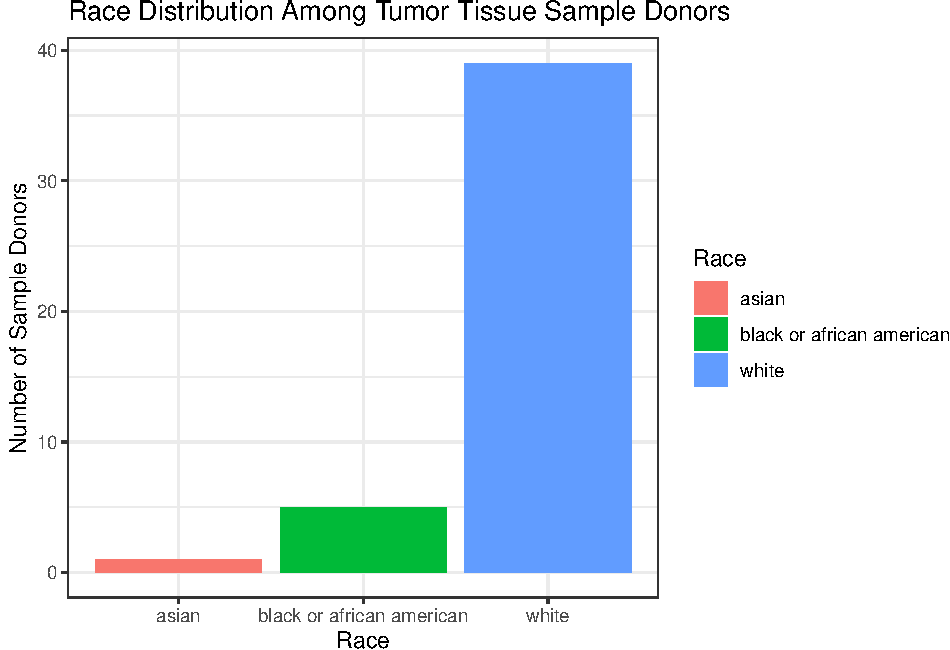
\includegraphics{LiuKevin_Final_Project_files/figure-latex/unnamed-chunk-5-1.pdf}

\newpage

\begin{Shaded}
\begin{Highlighting}[]
\CommentTok{\# plot bar plot among tumor tissue sample donors in terms of gender}
\NormalTok{sample\_metadata }\SpecialCharTok{\%\textgreater{}\%} 
  \FunctionTok{filter}\NormalTok{(}\SpecialCharTok{!}\FunctionTok{is.na}\NormalTok{(gender)) }\SpecialCharTok{\%\textgreater{}\%} \CommentTok{\# filter out gender with NAs (solid tissue normal samples)}
  \FunctionTok{ggplot}\NormalTok{() }\SpecialCharTok{+}
  \FunctionTok{geom\_bar}\NormalTok{(}\FunctionTok{aes}\NormalTok{(}\AttributeTok{x =}\NormalTok{ gender, }\AttributeTok{fill =}\NormalTok{ gender)) }\SpecialCharTok{+}
  \FunctionTok{theme\_bw}\NormalTok{() }\SpecialCharTok{+}
  \FunctionTok{labs}\NormalTok{(}\AttributeTok{x =} \StringTok{"Sex"}\NormalTok{, }\AttributeTok{y =} \StringTok{"Number of Sample Donors"}\NormalTok{, }\AttributeTok{fill =} \StringTok{"Sex"}\NormalTok{,}
       \AttributeTok{title =} \StringTok{"Sex Distribution Among Tumor Tissue Sample Donors"}\NormalTok{)}
\end{Highlighting}
\end{Shaded}

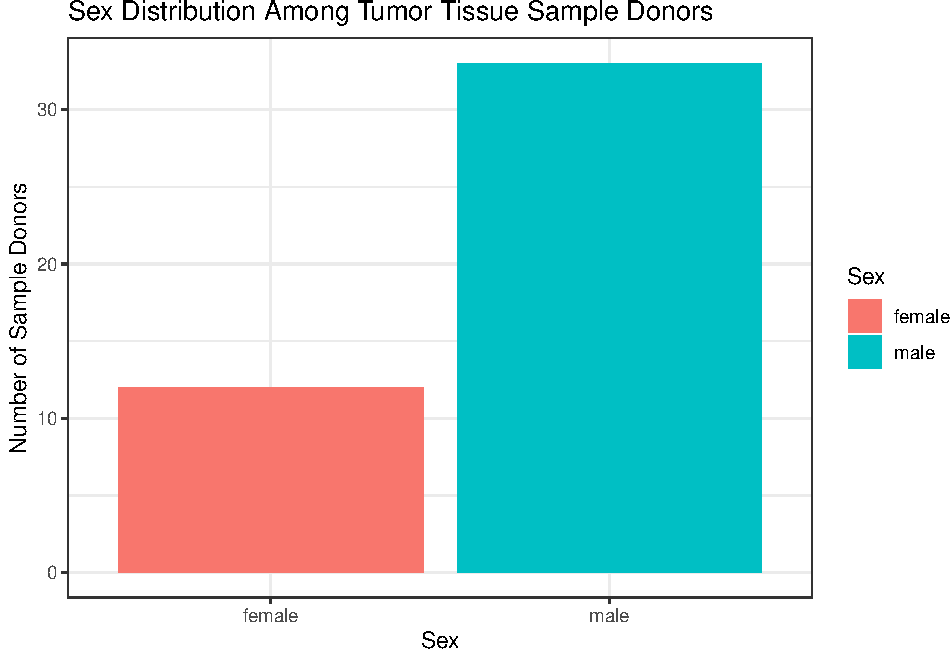
\includegraphics{LiuKevin_Final_Project_files/figure-latex/unnamed-chunk-6-1.pdf}

\newpage

\begin{Shaded}
\begin{Highlighting}[]
\CommentTok{\# plot bar plot among tumor tissue sample donors in terms of age groups}
\NormalTok{sample\_metadata }\SpecialCharTok{\%\textgreater{}\%} 
  \FunctionTok{filter}\NormalTok{(age\_group }\SpecialCharTok{!=} \StringTok{"Unknown"}\NormalTok{) }\SpecialCharTok{\%\textgreater{}\%} \CommentTok{\# filter out age group with NAs (solid tissue normal)}
  \FunctionTok{ggplot}\NormalTok{() }\SpecialCharTok{+}
  \FunctionTok{geom\_bar}\NormalTok{(}\FunctionTok{aes}\NormalTok{(}\AttributeTok{x =}\NormalTok{ age\_group, }\AttributeTok{fill =}\NormalTok{ age\_group)) }\SpecialCharTok{+}
  \FunctionTok{theme\_bw}\NormalTok{() }\SpecialCharTok{+}
  \FunctionTok{labs}\NormalTok{(}\AttributeTok{x =} \StringTok{"Age Group"}\NormalTok{, }\AttributeTok{y =} \StringTok{"Number of Sample Donors"}\NormalTok{, }\AttributeTok{fill =} \StringTok{"Age Group"}\NormalTok{,}
       \AttributeTok{title =} \StringTok{"Age Group Distribution Among Tumor Tissue Sample Donors"}\NormalTok{)}
\end{Highlighting}
\end{Shaded}

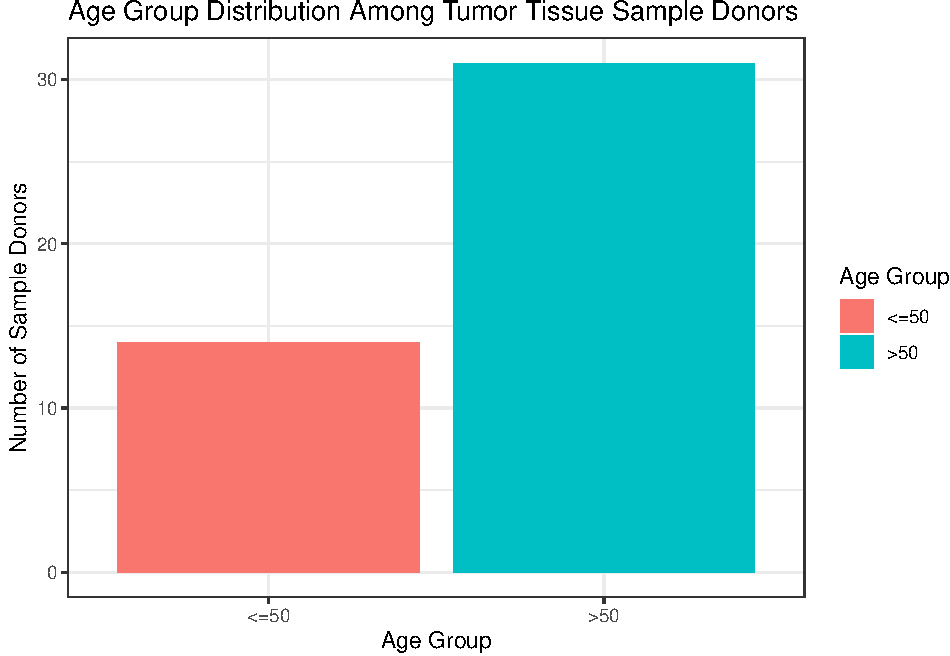
\includegraphics{LiuKevin_Final_Project_files/figure-latex/unnamed-chunk-7-1.pdf}

\newpage

\begin{Shaded}
\begin{Highlighting}[]
\CommentTok{\# plot bar plot among all tissue sample donors in terms of tissue source site}
\NormalTok{sample\_metadata }\SpecialCharTok{\%\textgreater{}\%} 
  \CommentTok{\# count how many sample subtypes per tissue source site}
\NormalTok{  dplyr}\SpecialCharTok{::}\FunctionTok{count}\NormalTok{(paper\_Tissue.source.site, sample\_subtype, }\AttributeTok{name =} \StringTok{"count"}\NormalTok{) }\SpecialCharTok{\%\textgreater{}\%} 
  \FunctionTok{ggplot}\NormalTok{() }\SpecialCharTok{+}
  \FunctionTok{geom\_bar}\NormalTok{(}\FunctionTok{aes}\NormalTok{(}\AttributeTok{x =}\NormalTok{ paper\_Tissue.source.site, }\AttributeTok{y =}\NormalTok{ count, }\AttributeTok{fill =}\NormalTok{ sample\_subtype), }\AttributeTok{stat =} \StringTok{"identity"}\NormalTok{) }\SpecialCharTok{+}
  \FunctionTok{theme\_bw}\NormalTok{() }\SpecialCharTok{+}
  \FunctionTok{labs}\NormalTok{(}\AttributeTok{x =} \StringTok{"Tissue Source Site"}\NormalTok{, }\AttributeTok{y =} \StringTok{"Number of Sample Donors"}\NormalTok{, }\AttributeTok{fill =} \StringTok{"Sample Subtype"}\NormalTok{,}
       \AttributeTok{title =} \StringTok{"Distribution of Tissue Source Site Among All Tissue Sample Donors"}\NormalTok{) }\SpecialCharTok{+}
  \FunctionTok{theme}\NormalTok{(}\AttributeTok{axis.text.x =} \FunctionTok{element\_text}\NormalTok{(}\AttributeTok{angle =} \DecValTok{45}\NormalTok{, }\AttributeTok{hjust =} \DecValTok{1}\NormalTok{, }\AttributeTok{vjust =} \DecValTok{1}\NormalTok{))}
\end{Highlighting}
\end{Shaded}

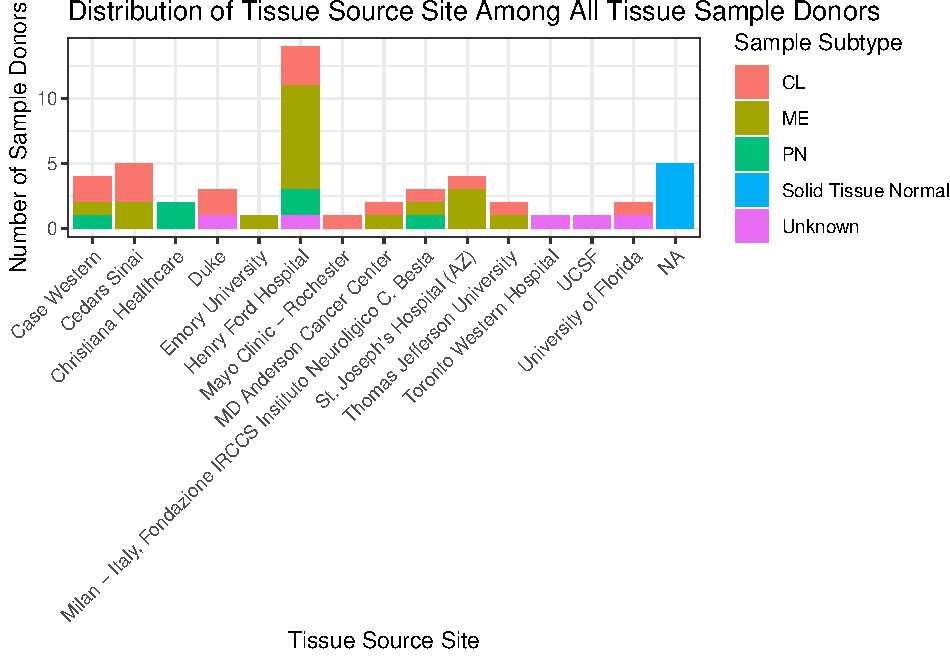
\includegraphics{LiuKevin_Final_Project_files/figure-latex/unnamed-chunk-8-1.pdf}

\newpage

\begin{Shaded}
\begin{Highlighting}[]
\CommentTok{\# plot box plot among tumor tissue sample donors in terms of age, survival years, }
\CommentTok{\# and age at diagnosis}
\NormalTok{sample\_metadata }\SpecialCharTok{\%\textgreater{}\%} 
  \FunctionTok{select}\NormalTok{(sample\_subtype, }\FunctionTok{all\_of}\NormalTok{(num\_demographic\_vars)) }\SpecialCharTok{\%\textgreater{}\%} 
  \FunctionTok{mutate}\NormalTok{(}\AttributeTok{survival\_years =}\NormalTok{ paper\_Survival..months. }\SpecialCharTok{/}\DecValTok{12}\NormalTok{) }\SpecialCharTok{\%\textgreater{}\%} 
  \FunctionTok{pivot\_longer}\NormalTok{(}\AttributeTok{cols =} \FunctionTok{c}\NormalTok{(age\_at\_index, survival\_years, paper\_Age..years.at.diagnosis.)) }\SpecialCharTok{\%\textgreater{}\%} 
  \FunctionTok{filter}\NormalTok{(}\SpecialCharTok{!}\FunctionTok{is.na}\NormalTok{(value)) }\SpecialCharTok{\%\textgreater{}\%} \CommentTok{\# filter out data with NAs (solid tissue normal)}
  \FunctionTok{ggplot}\NormalTok{() }\SpecialCharTok{+}
  \FunctionTok{geom\_boxplot}\NormalTok{(}\FunctionTok{aes}\NormalTok{(}\AttributeTok{x =}\NormalTok{ sample\_subtype, }\AttributeTok{y =}\NormalTok{ value, }\AttributeTok{fill =}\NormalTok{ sample\_subtype),}
               \AttributeTok{outlier.shape =} \ConstantTok{NA}\NormalTok{) }\SpecialCharTok{+} \CommentTok{\# remove outlier plots to avoid double{-}plotting}
  \FunctionTok{geom\_jitter}\NormalTok{(}\FunctionTok{aes}\NormalTok{(}\AttributeTok{x =}\NormalTok{ sample\_subtype, }\AttributeTok{y =}\NormalTok{ value)) }\SpecialCharTok{+}
  \FunctionTok{theme\_bw}\NormalTok{() }\SpecialCharTok{+}
  \FunctionTok{labs}\NormalTok{(}\AttributeTok{x =} \StringTok{"Sample Subtype"}\NormalTok{, }\AttributeTok{y =} \StringTok{"Number of Years"}\NormalTok{, }\AttributeTok{fill =} \StringTok{"Sample Subtype"}\NormalTok{,}
       \AttributeTok{title =} \StringTok{"Distribution of Age and Survival in Years for Tumor Tissue Sample Donors"}\NormalTok{) }\SpecialCharTok{+}
  \FunctionTok{facet\_wrap}\NormalTok{(}\SpecialCharTok{\textasciitilde{}}\NormalTok{name, }\AttributeTok{scales =} \StringTok{"free"}\NormalTok{)}
\end{Highlighting}
\end{Shaded}

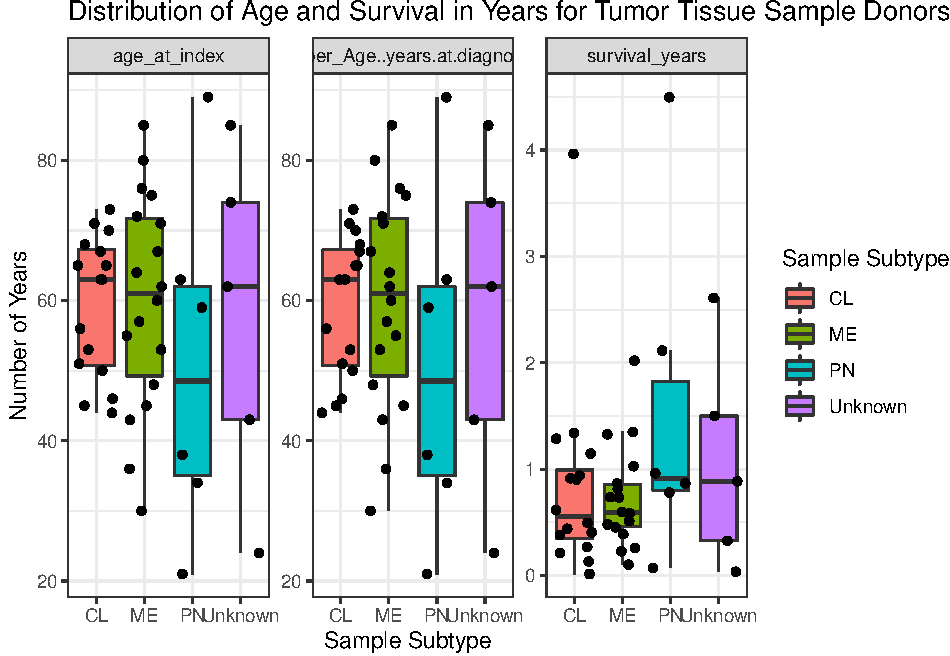
\includegraphics{LiuKevin_Final_Project_files/figure-latex/unnamed-chunk-9-1.pdf}

Based on the above plots, it is apparent that our dataset is biased
towards having a majority of sample donors who are white, male, and age
greater than 50 years. We Additionally observe that Henry Ford Hospital
contributed the largest number of samples and that donors with the PN
sample subtype are typically younger in terms of age at index and age of
diagnosis; these individuals also appear to have a longer survival time
in years, which is expected given their young age and earlier diagnosis.

\newpage

\hypertarget{pca-for-identification-of-prognostic-pathogenic-genes-in-gbm}{%
\section{PCA for Identification of Prognostic Pathogenic Genes in
GBM}\label{pca-for-identification-of-prognostic-pathogenic-genes-in-gbm}}

As stated in the project overview, we hypothesize that PCA can be used
to distinguish the prognostic pathogenic genes from our 24 candidate
immune genes. Here, we will perform the PCA on our normalized and
filtered RNA-seq read count matrix and attempt to interpret the PCA
weights in hopes that it will inform us of the prognostic pathogenic
genes of interest that were identified by Liang et al.

\hypertarget{determine-number-of-pcs-needed-to-explain-at-least-90-variance}{%
\subsection{Determine number of PCs needed to explain at least 90\%
variance}\label{determine-number-of-pcs-needed-to-explain-at-least-90-variance}}

First, we will define a function that computes the number of PCs needed
to account for at least 90\% variance, which may inform us of the number
of PCs to be used in subsequent analyses. We will then compute the PCA
object, apply our function to determine the number of PCs needed to
account for 90\% variance, and inspect the percent variance accounted
for by each PC.

\begin{Shaded}
\begin{Highlighting}[]
\CommentTok{\# function that indicates how many PCs needed for 90\% variance}
\NormalTok{n\_pc }\OtherTok{=} \ControlFlowTok{function}\NormalTok{(pr)\{}
\NormalTok{  pr\_var\_exp }\OtherTok{=}\NormalTok{ pr}\SpecialCharTok{$}\NormalTok{sdev}\SpecialCharTok{\^{}}\DecValTok{2}\SpecialCharTok{/}\FunctionTok{sum}\NormalTok{(pr}\SpecialCharTok{$}\NormalTok{sdev}\SpecialCharTok{\^{}}\DecValTok{2}\NormalTok{)}
\NormalTok{  var\_exp\_tot }\OtherTok{=} \DecValTok{0}
\NormalTok{  pc\_count }\OtherTok{=} \DecValTok{0}
  
  \ControlFlowTok{for}\NormalTok{(i }\ControlFlowTok{in} \DecValTok{1}\SpecialCharTok{:}\FunctionTok{length}\NormalTok{(pr\_var\_exp))\{}
    \ControlFlowTok{if}\NormalTok{(var\_exp\_tot }\SpecialCharTok{\textless{}} \FloatTok{0.9}\NormalTok{)\{}
\NormalTok{      var\_exp\_tot }\OtherTok{=}\NormalTok{ var\_exp\_tot }\SpecialCharTok{+}\NormalTok{ pr\_var\_exp[i]}
\NormalTok{      pc\_count }\OtherTok{=}\NormalTok{ pc\_count }\SpecialCharTok{+} \DecValTok{1}
\NormalTok{      \}}
\NormalTok{    \}}
  
  \FunctionTok{return}\NormalTok{(pc\_count)}
\NormalTok{\}}

\CommentTok{\# create PCA object on transposed counts matrix after scaling and centering the data}
\NormalTok{count\_pca }\OtherTok{=} \FunctionTok{prcomp}\NormalTok{(}\FunctionTok{t}\NormalTok{(GBMMatrix\_norm\_filter), }\AttributeTok{scale. =} \ConstantTok{TRUE}\NormalTok{, }\AttributeTok{center =} \ConstantTok{TRUE}\NormalTok{)}

\CommentTok{\# compute number of PCs needed to account for 90\% variance}
\FunctionTok{n\_pc}\NormalTok{(count\_pca) }\CommentTok{\# needs 12 PCs to account for 90\% variance}
\end{Highlighting}
\end{Shaded}

\begin{verbatim}
## [1] 12
\end{verbatim}

\begin{Shaded}
\begin{Highlighting}[]
\CommentTok{\# inspect how much variance each PC explains}
\NormalTok{count\_pca}\SpecialCharTok{$}\NormalTok{sdev}\SpecialCharTok{\^{}}\DecValTok{2}\SpecialCharTok{/}\FunctionTok{sum}\NormalTok{(count\_pca}\SpecialCharTok{$}\NormalTok{sdev}\SpecialCharTok{\^{}}\DecValTok{2}\NormalTok{)}
\end{Highlighting}
\end{Shaded}

\begin{verbatim}
##  [1] 0.436595429 0.107658357 0.079536937 0.060410524 0.042822935 0.038803455
##  [7] 0.032756539 0.027324232 0.026520806 0.022574195 0.021318769 0.020245674
## [13] 0.014396656 0.012946540 0.012212993 0.009164719 0.006982328 0.006332617
## [19] 0.005873127 0.004573318 0.003491596 0.003028238 0.002901954 0.001528061
\end{verbatim}

As shown above, we will need 12 PCs to account for at least 90\%
variance. Our first PC accounts for 43.7\% of variance and our second PC
accounts for 10.8\% of variance.

\newpage

\hypertarget{scree-plot-of-pca-variance-explained-per-pc}{%
\subsection{Scree plot of PCA variance explained per
PC}\label{scree-plot-of-pca-variance-explained-per-pc}}

To visually inspect the amount of variance explained per PC, we will
plot a scree plot as shown below.

\begin{Shaded}
\begin{Highlighting}[]
\CommentTok{\# create a sequentially numbered dataframe of variances explained per PC and plot scree plot}
\FunctionTok{data.frame}\NormalTok{(}\AttributeTok{PC =} \FunctionTok{seq}\NormalTok{(}\DecValTok{1}\NormalTok{, }\FunctionTok{ncol}\NormalTok{(count\_pca}\SpecialCharTok{$}\NormalTok{x)), }
           \AttributeTok{var\_explained =}\NormalTok{ (count\_pca}\SpecialCharTok{$}\NormalTok{sdev}\SpecialCharTok{\^{}}\DecValTok{2}\SpecialCharTok{/}\FunctionTok{sum}\NormalTok{(count\_pca}\SpecialCharTok{$}\NormalTok{sdev}\SpecialCharTok{\^{}}\DecValTok{2}\NormalTok{))}\SpecialCharTok{*}\DecValTok{100}\NormalTok{) }\SpecialCharTok{\%\textgreater{}\%} 
  \FunctionTok{ggplot}\NormalTok{(}\FunctionTok{aes}\NormalTok{(}\AttributeTok{x =} \FunctionTok{factor}\NormalTok{(PC), }\AttributeTok{y =}\NormalTok{ var\_explained)) }\SpecialCharTok{+} \CommentTok{\# make PC a factor so axis ticks match each bar}
  \FunctionTok{geom\_bar}\NormalTok{(}\AttributeTok{stat =} \StringTok{"identity"}\NormalTok{) }\SpecialCharTok{+} 
  \FunctionTok{theme\_bw}\NormalTok{() }\SpecialCharTok{+}
  \FunctionTok{labs}\NormalTok{(}\AttributeTok{x =} \StringTok{"PC"}\NormalTok{, }\AttributeTok{y =} \StringTok{"Percent Variance Explained"}\NormalTok{, }\AttributeTok{title =} \StringTok{"Scree plot"}\NormalTok{)}
\end{Highlighting}
\end{Shaded}

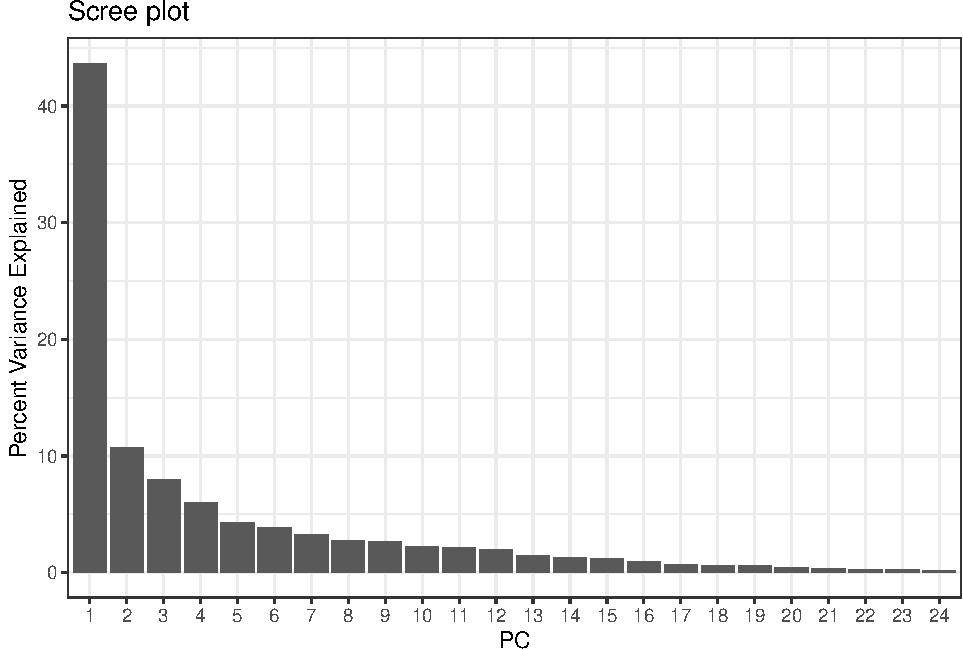
\includegraphics{LiuKevin_Final_Project_files/figure-latex/unnamed-chunk-11-1.pdf}

\newpage

\hypertarget{scatter-plots-of-pca-rotated-data-points}{%
\subsection{Scatter plots of PCA rotated data
points}\label{scatter-plots-of-pca-rotated-data-points}}

We hypothesized that the differential gene expression between normal
tissue samples and tumor tissue samples (i.e., Solid Tissue Normal and
Primary Tumor) will be the main driving factor influencing our PCs.
Here, we will plot the first two PCs as a scatter plot and color them by
either sample subtype or sample type to see if the respective data
points group together nicely.

\begin{Shaded}
\begin{Highlighting}[]
\CommentTok{\# merge PCA scores with sample metadata for plotting}
\NormalTok{sample\_metadata\_pca }\OtherTok{=} \FunctionTok{data.frame}\NormalTok{(count\_pca}\SpecialCharTok{$}\NormalTok{x) }\SpecialCharTok{\%\textgreater{}\%} 
  \FunctionTok{merge}\NormalTok{(sample\_metadata, }\AttributeTok{by =} \StringTok{"row.names"}\NormalTok{) }\SpecialCharTok{\%\textgreater{}\%} 
  \FunctionTok{column\_to\_rownames}\NormalTok{(}\StringTok{"Row.names"}\NormalTok{)}

\CommentTok{\# plot PC1 and PC2 as scatter plots, colored and faceted by sample subtype and diagnosis}
\NormalTok{sample\_metadata\_pca }\SpecialCharTok{\%\textgreater{}\%} 
  \FunctionTok{select}\NormalTok{(sample\_type, sample\_subtype, PC1, PC2) }\SpecialCharTok{\%\textgreater{}\%} 
  \FunctionTok{pivot\_longer}\NormalTok{(}\AttributeTok{cols =} \FunctionTok{c}\NormalTok{(sample\_type, sample\_subtype)) }\SpecialCharTok{\%\textgreater{}\%} 
  \FunctionTok{ggplot}\NormalTok{() }\SpecialCharTok{+}
  \FunctionTok{geom\_point}\NormalTok{(}\FunctionTok{aes}\NormalTok{(}\AttributeTok{x =}\NormalTok{ PC1, }\AttributeTok{y =}\NormalTok{ PC2, }\AttributeTok{color =}\NormalTok{ value)) }\SpecialCharTok{+}
  \FunctionTok{theme\_bw}\NormalTok{() }\SpecialCharTok{+}
  \FunctionTok{facet\_wrap}\NormalTok{(}\SpecialCharTok{\textasciitilde{}}\NormalTok{name) }\SpecialCharTok{+}
  \FunctionTok{theme}\NormalTok{(}\AttributeTok{aspect.ratio =} \DecValTok{1}\NormalTok{) }\SpecialCharTok{+}
  \FunctionTok{labs}\NormalTok{(}\AttributeTok{color =} \StringTok{"Sample Type/Subtype"}\NormalTok{, }
       \AttributeTok{title =} \StringTok{"Scatter plot of PC1 and PC2 colored by sample subtype and sample type"}\NormalTok{)}
\end{Highlighting}
\end{Shaded}

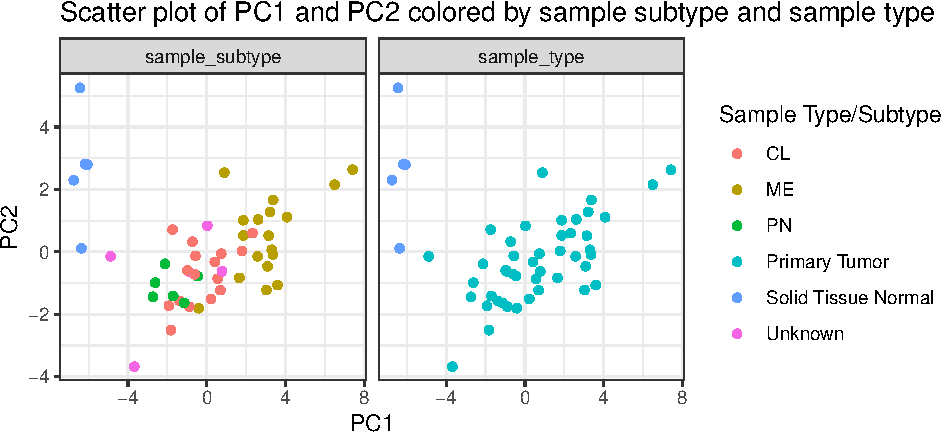
\includegraphics{LiuKevin_Final_Project_files/figure-latex/unnamed-chunk-12-1.pdf}

Based on the above plot, it seems like our hypothesis is mostly correct:
when colored by sample type (i.e., normal tissue samples and tumor
tissue samples), the two groups of data points group together nicely;
when colored by sample subtype, the Solid Tissue Normal samples are
clearly distinguished from the tumor tissue samples while the subtypes
are largely mixed together and cannot be distinguished.

\newpage

\hypertarget{bar-plots-of-pca-weights-to-determine-gene-relevance-of-pc1-and-pc2}{%
\subsection{Bar plots of PCA weights to determine gene relevance of PC1
and
PC2}\label{bar-plots-of-pca-weights-to-determine-gene-relevance-of-pc1-and-pc2}}

Next, we will make bar plots of the PCA weights for PC1 and PC2 to
determine the contribution of each gene to the weight of rotation that
gives rise to our respective PCA scores. We expect that the prognostic
pathogenic genes to have the most extreme values in either PC1 or PC2 as
they should contribute the most to each component.

\begin{Shaded}
\begin{Highlighting}[]
\CommentTok{\# plot the weights of PC1 as bar plots, using gene names instead of gene codes}
\FunctionTok{data.frame}\NormalTok{(count\_pca}\SpecialCharTok{$}\NormalTok{rotation) }\SpecialCharTok{\%\textgreater{}\%} 
  \FunctionTok{mutate}\NormalTok{(}\AttributeTok{gene\_name =}\NormalTok{ gene\_metadata }\SpecialCharTok{\%\textgreater{}\%} \FunctionTok{select}\NormalTok{(gene\_name) }\SpecialCharTok{\%\textgreater{}\%} \FunctionTok{as\_vector}\NormalTok{()) }\SpecialCharTok{\%\textgreater{}\%} 
  \FunctionTok{ggplot}\NormalTok{(}\FunctionTok{aes}\NormalTok{(}\AttributeTok{x =}\NormalTok{ gene\_name, }\AttributeTok{y =}\NormalTok{ PC1)) }\SpecialCharTok{+}
  \FunctionTok{geom\_bar}\NormalTok{(}\AttributeTok{stat =} \StringTok{"identity"}\NormalTok{) }\SpecialCharTok{+}
  \FunctionTok{theme\_bw}\NormalTok{() }\SpecialCharTok{+}
  \FunctionTok{theme}\NormalTok{(}\AttributeTok{axis.text.x =} \FunctionTok{element\_text}\NormalTok{(}\AttributeTok{angle =} \DecValTok{45}\NormalTok{, }\AttributeTok{vjust =} \DecValTok{1}\NormalTok{, }\AttributeTok{hjust =} \DecValTok{1}\NormalTok{)) }\SpecialCharTok{+}
  \FunctionTok{labs}\NormalTok{(}\AttributeTok{x =} \StringTok{"Gene Name"}\NormalTok{, }\AttributeTok{title =} \StringTok{"PC1 Weights"}\NormalTok{)}
\end{Highlighting}
\end{Shaded}

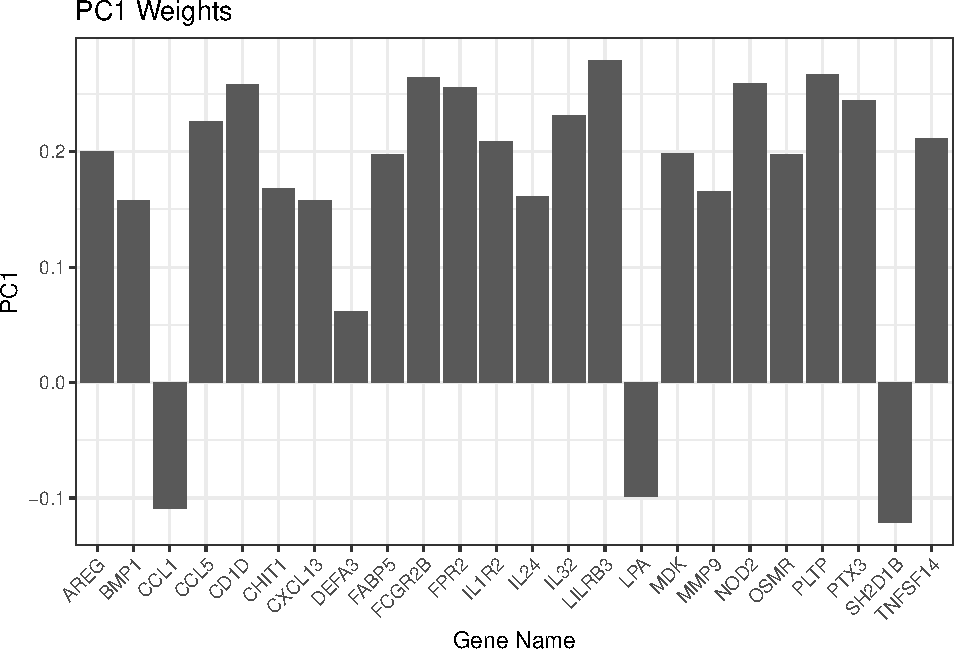
\includegraphics{LiuKevin_Final_Project_files/figure-latex/unnamed-chunk-13-1.pdf}

\begin{Shaded}
\begin{Highlighting}[]
\CommentTok{\# plot the weights of PC2 as bar plots, using gene names instead of gene codes}
\FunctionTok{data.frame}\NormalTok{(count\_pca}\SpecialCharTok{$}\NormalTok{rotation) }\SpecialCharTok{\%\textgreater{}\%} 
  \FunctionTok{mutate}\NormalTok{(}\AttributeTok{gene\_name =}\NormalTok{ gene\_metadata }\SpecialCharTok{\%\textgreater{}\%} \FunctionTok{select}\NormalTok{(gene\_name) }\SpecialCharTok{\%\textgreater{}\%} \FunctionTok{as\_vector}\NormalTok{()) }\SpecialCharTok{\%\textgreater{}\%} 
  \FunctionTok{ggplot}\NormalTok{(}\FunctionTok{aes}\NormalTok{(}\AttributeTok{x =}\NormalTok{ gene\_name, }\AttributeTok{y =}\NormalTok{ PC2)) }\SpecialCharTok{+}
  \FunctionTok{geom\_bar}\NormalTok{(}\AttributeTok{stat =} \StringTok{"identity"}\NormalTok{) }\SpecialCharTok{+}
  \FunctionTok{theme\_bw}\NormalTok{() }\SpecialCharTok{+}
  \FunctionTok{theme}\NormalTok{(}\AttributeTok{axis.text.x =} \FunctionTok{element\_text}\NormalTok{(}\AttributeTok{angle =} \DecValTok{45}\NormalTok{, }\AttributeTok{vjust =} \DecValTok{1}\NormalTok{, }\AttributeTok{hjust =} \DecValTok{1}\NormalTok{)) }\SpecialCharTok{+}
  \FunctionTok{labs}\NormalTok{(}\AttributeTok{x =} \StringTok{"Gene Name"}\NormalTok{, }\AttributeTok{title =} \StringTok{"PC2 Weights"}\NormalTok{)}
\end{Highlighting}
\end{Shaded}

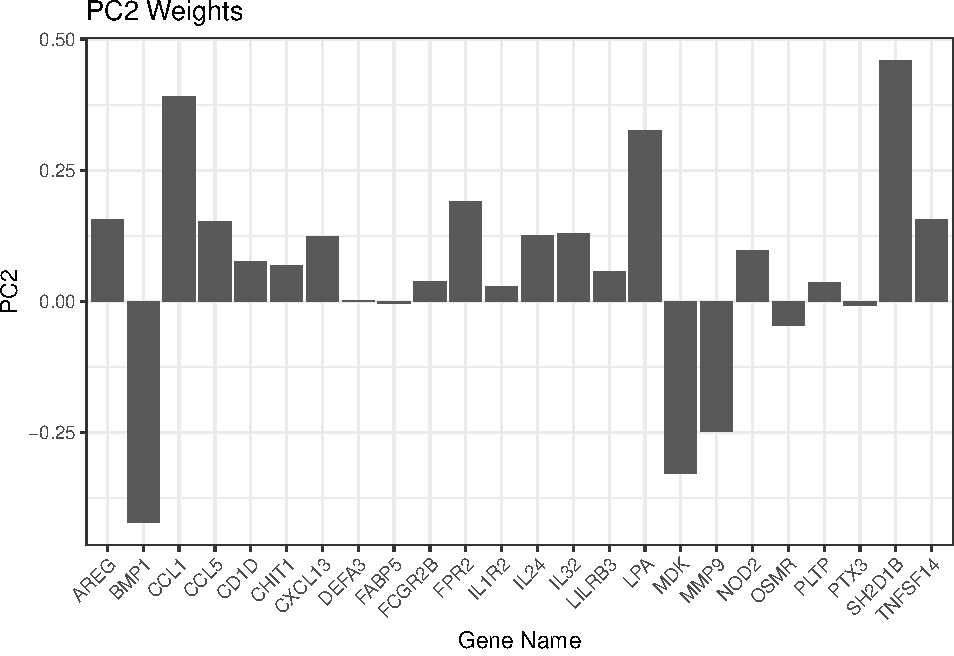
\includegraphics{LiuKevin_Final_Project_files/figure-latex/unnamed-chunk-13-2.pdf}

It is evident based on the above two plots that CCL1, LPA, and SH2D1B
are consistently giving most extreme weights for PC1 and PC2. This is
consistent with the identified prognostic pathogenic genes by Liang et
al.~and supports our hypothesis.

\newpage

\hypertarget{hierarchical-clustering-of-immune-gene-counts}{%
\section{Hierarchical Clustering of Immune Gene
Counts}\label{hierarchical-clustering-of-immune-gene-counts}}

Next, we will perform hierarchical clustering on all 24 immune genes
identified by Liang et al.~as well as all samples to see if there are
any relationships between genes and between samples based on their gene
expression profiles.

We will first cluster on genes across samples using euclidean distance
and complete linkage to give the most compact clusters.

\begin{Shaded}
\begin{Highlighting}[]
\FunctionTok{set.seed}\NormalTok{(}\DecValTok{713}\NormalTok{) }\CommentTok{\# set seed to 713 for reproducibility of clustering}

\CommentTok{\# create hierarchical clustering object of genes using complete linkage method }
\CommentTok{\# after scaling the counts matrix and calculating the euclidean distances}
\NormalTok{gene\_hclust }\OtherTok{=}\NormalTok{ GBMMatrix\_norm\_filter }\SpecialCharTok{\%\textgreater{}\%} 
  \FunctionTok{scale}\NormalTok{() }\SpecialCharTok{\%\textgreater{}\%} 
  \FunctionTok{dist}\NormalTok{(}\AttributeTok{method =} \StringTok{"euclidean"}\NormalTok{) }\SpecialCharTok{\%\textgreater{}\%} 
  \FunctionTok{hclust}\NormalTok{(}\AttributeTok{method =} \StringTok{"complete"}\NormalTok{)}

\FunctionTok{plot}\NormalTok{(gene\_hclust) }\CommentTok{\# plot the cluster dendrogram}
\end{Highlighting}
\end{Shaded}

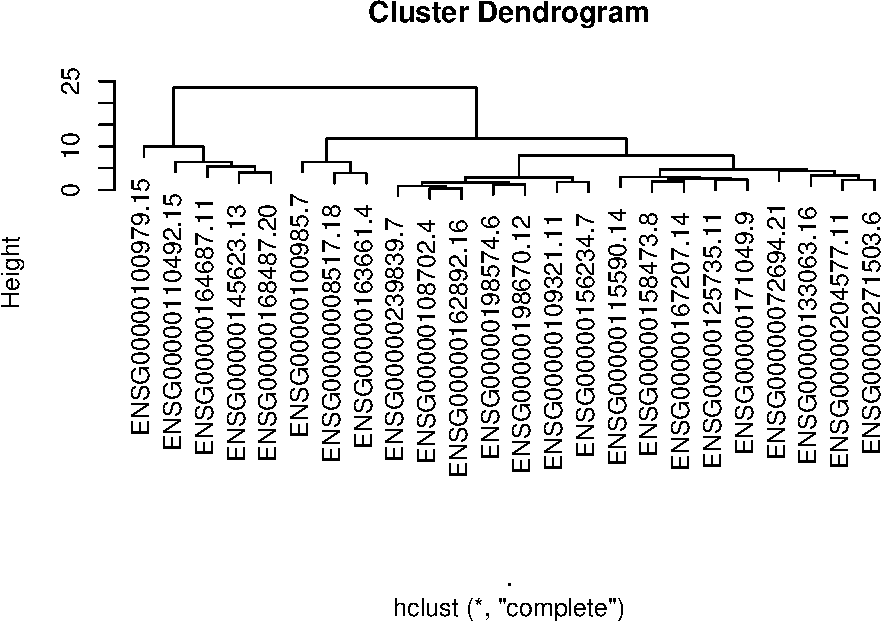
\includegraphics{LiuKevin_Final_Project_files/figure-latex/unnamed-chunk-14-1.pdf}

\begin{Shaded}
\begin{Highlighting}[]
\CommentTok{\# cut the dendrogram into 5 clusters after visual inspection of dendrogram and }
\CommentTok{\# store as dataframe}
\NormalTok{gene\_clusters }\OtherTok{=} \FunctionTok{data.frame}\NormalTok{(}\AttributeTok{clusters =} \FunctionTok{cutree}\NormalTok{(gene\_hclust, }\AttributeTok{k =} \DecValTok{5}\NormalTok{))}
\end{Highlighting}
\end{Shaded}

Here, we decided to cut the dendrogram into 5 clusters of genes as these
clusters (visually) convey the most relevance between genes without
leaving too many single genes in their own clusters.

\newpage

We will repeat the above process for samples across genes. This time, we
are attempting to cluster samples of the same subtype together since we
expect that similar subtypes should have similar gene expression
profiles. For plotting purposes, this will be done by concatenating
together the sample ID with each sample's subtype.

\begin{Shaded}
\begin{Highlighting}[]
\FunctionTok{set.seed}\NormalTok{(}\DecValTok{713}\NormalTok{) }\CommentTok{\# set seed to 713 for reproducibility of clustering}

\CommentTok{\# create a hierarchical clustering dendrogram of individuals and their subtypes}
\NormalTok{GBMMatrix\_norm\_filter }\SpecialCharTok{\%\textgreater{}\%} 
  \FunctionTok{t}\NormalTok{() }\SpecialCharTok{\%\textgreater{}\%} \CommentTok{\# transpose the matrix so sample IDs are rows for merging with sample metadata}
  \FunctionTok{merge}\NormalTok{(sample\_metadata }\SpecialCharTok{\%\textgreater{}\%} \FunctionTok{select}\NormalTok{(sample\_subtype), }\AttributeTok{by =} \StringTok{"row.names"}\NormalTok{) }\SpecialCharTok{\%\textgreater{}\%}
  \FunctionTok{mutate}\NormalTok{(}\AttributeTok{Row.names =} \FunctionTok{str\_c}\NormalTok{(Row.names, }\StringTok{"\_"}\NormalTok{, sample\_subtype)) }\SpecialCharTok{\%\textgreater{}\%} \CommentTok{\# concat ID and subtypes}
  \FunctionTok{column\_to\_rownames}\NormalTok{(}\StringTok{"Row.names"}\NormalTok{) }\SpecialCharTok{\%\textgreater{}\%} \CommentTok{\# make the concatenated string the new row names}
  \FunctionTok{select}\NormalTok{(}\SpecialCharTok{{-}}\NormalTok{sample\_subtype) }\SpecialCharTok{\%\textgreater{}\%} \CommentTok{\# remove the sample subtype from the dataframe}
  \FunctionTok{as.matrix}\NormalTok{() }\SpecialCharTok{\%\textgreater{}\%} \CommentTok{\# convert counts dataframe to matrix}
  \FunctionTok{scale}\NormalTok{() }\SpecialCharTok{\%\textgreater{}\%} \CommentTok{\# scale the data}
  \FunctionTok{dist}\NormalTok{(}\AttributeTok{method =} \StringTok{"euclidean"}\NormalTok{) }\SpecialCharTok{\%\textgreater{}\%} \CommentTok{\# compute euclidean distances for clustering}
  \FunctionTok{hclust}\NormalTok{(}\AttributeTok{method =} \StringTok{"complete"}\NormalTok{) }\SpecialCharTok{\%\textgreater{}\%} \CommentTok{\# hierarchical clustering using complete linkage}
  \FunctionTok{plot}\NormalTok{(}\AttributeTok{cex =} \FloatTok{0.6}\NormalTok{) }\CommentTok{\# plot the dendrogram}
\end{Highlighting}
\end{Shaded}

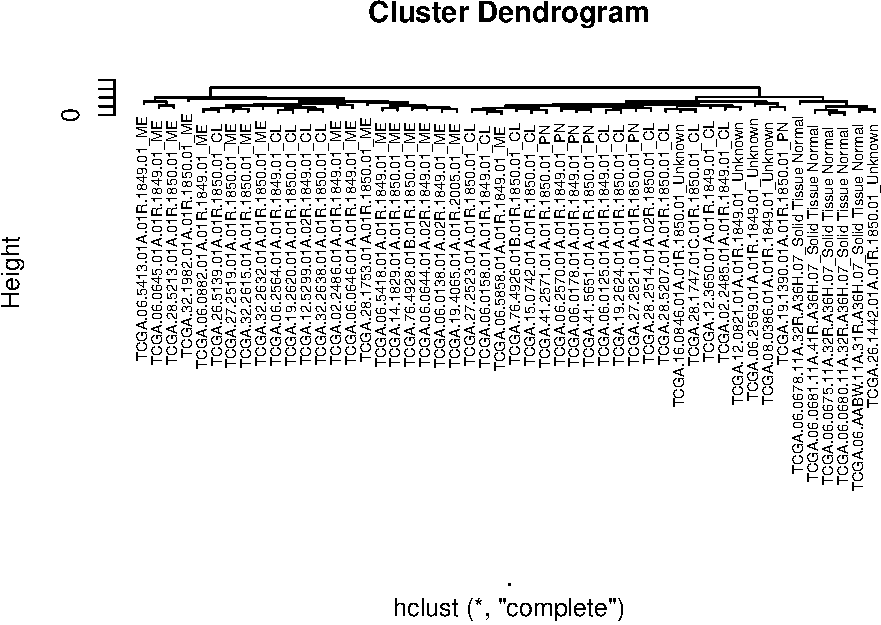
\includegraphics{LiuKevin_Final_Project_files/figure-latex/unnamed-chunk-15-1.pdf}

Given the above dendrogram, we will cut the dendrogram into 3 clusters:
(mostly) ME subtype, (mostly) Solid Tissue Normal subtype, and all
remaining subtypes that are mixed together. We did not perform the
cutting step here since we will create a heatmap of the clusters in the
next step.

\newpage

To better visualize the gene expression profiles of the 24 immune genes
relevant to the prognosis of GBM, we will create a heatmap that
incorporates hierarchical clustering based on the number of clusters we
have determined in the above steps both for genes across samples (rows)
and samples across genes (columns).

\begin{Shaded}
\begin{Highlighting}[]
\CommentTok{\# create a heatmap of gene expression levels and perform hierarchical clustering }
\CommentTok{\# on both individuals (columns) and genes (rows)}
\FunctionTok{pheatmap}\NormalTok{(GBMMatrix\_norm\_filter, }
         \AttributeTok{clustering\_method =} \StringTok{"complete"}\NormalTok{, }\CommentTok{\# use complete linkage method}
         \AttributeTok{clustering\_distance\_rows =} \StringTok{"euclidean"}\NormalTok{, }\CommentTok{\# use euclidean distance}
         \AttributeTok{clustering\_distance\_cols =} \StringTok{"euclidean"}\NormalTok{, }\CommentTok{\# use euclidean distance}
         \AttributeTok{fontsize =} \DecValTok{6}\NormalTok{, }
         \AttributeTok{cluster\_cols =} \ConstantTok{TRUE}\NormalTok{, }\AttributeTok{cluster\_rows =} \ConstantTok{TRUE}\NormalTok{, }\CommentTok{\# hclust on both rows and columns}
         \AttributeTok{cutree\_cols =} \DecValTok{3}\NormalTok{, }\AttributeTok{cutree\_rows =} \DecValTok{5}\NormalTok{, }\CommentTok{\# cut into number of clusters}
         \AttributeTok{labels\_row =}\NormalTok{ gene\_metadata }\SpecialCharTok{\%\textgreater{}\%} \FunctionTok{select}\NormalTok{(gene\_name) }\SpecialCharTok{\%\textgreater{}\%} \FunctionTok{as\_vector}\NormalTok{(), }\CommentTok{\# show gene names}
         \AttributeTok{annotation\_col =}\NormalTok{ sample\_metadata }\SpecialCharTok{\%\textgreater{}\%} \FunctionTok{select}\NormalTok{(sample\_subtype), }\CommentTok{\# indicate subtype}
         \AttributeTok{annotation\_row =}\NormalTok{ gene\_clusters, }\CommentTok{\# indicate gene clusters}
         \AttributeTok{show\_colnames =} \ConstantTok{FALSE}\NormalTok{) }\CommentTok{\# don\textquotesingle{}t show sample names}
\end{Highlighting}
\end{Shaded}

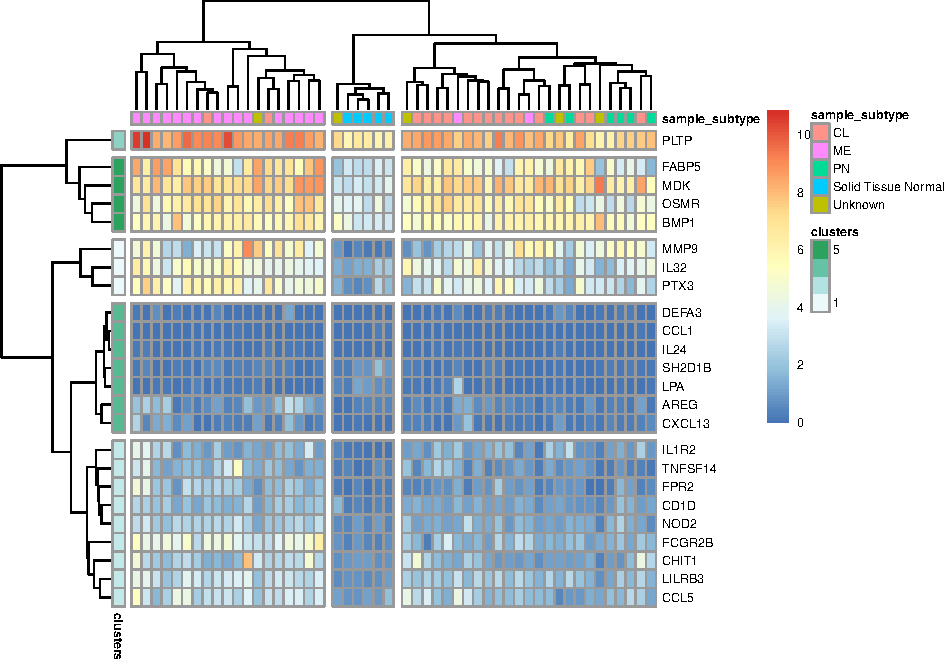
\includegraphics{LiuKevin_Final_Project_files/figure-latex/unnamed-chunk-16-1.pdf}

It is deeply satisfying to see our resulting heatmap--data is beautiful!
Based on our previously determined number of clusters for both genes and
samples, we see that samples of normal tissue have much lower expression
levels of almost all genes except DEFA3, CCL1, IL24, AREG, and CXCL13
while these samples express higher levels of SH2D1B and LPA relative to
GBM tissue samples. We also see that when clustering on samples (i.e.,
columns), the ME subtype and Solid Tissue Normal subtype are nicely
clustered together in their respective clusters.

\newpage

\hypertarget{verification-of-observed-trends-identified-by-liang-et-al.-2020}{%
\section{Verification of Observed Trends Identified by Liang et
al.~(2020)}\label{verification-of-observed-trends-identified-by-liang-et-al.-2020}}

Finally, we attempt to replicate the observed trends identified by Liang
et al.~Based on their results, CCL1 is expressed at higher levels in
males relative to females while BMP1 and OSMR are expressed at higher
levels in those with ages \textgreater50yo. We will accomplish this by
creating box plots of the respective observations.

\begin{Shaded}
\begin{Highlighting}[]
\CommentTok{\# make a copy of the counts matrix with gene name as the row names and merge in }
\CommentTok{\# sample metadata for plotting}
\NormalTok{gene\_sample }\OtherTok{=}\NormalTok{ GBMMatrix\_norm\_filter }\SpecialCharTok{\%\textgreater{}\%} 
  \CommentTok{\# merge gene metadata containing only the gene names by the row names}
  \FunctionTok{merge}\NormalTok{(gene\_metadata }\SpecialCharTok{\%\textgreater{}\%} \FunctionTok{select}\NormalTok{(gene\_name), }\AttributeTok{by =} \StringTok{"row.names"}\NormalTok{) }\SpecialCharTok{\%\textgreater{}\%} 
  \FunctionTok{column\_to\_rownames}\NormalTok{(}\StringTok{"gene\_name"}\NormalTok{) }\SpecialCharTok{\%\textgreater{}\%} \CommentTok{\# make the gene name the row names}
  \CommentTok{\# remove the original row names that was forced into a column when forcing matrix }
  \CommentTok{\# into dataframe}
  \FunctionTok{select}\NormalTok{(}\SpecialCharTok{{-}}\NormalTok{Row.names) }\SpecialCharTok{\%\textgreater{}\%} 
  \FunctionTok{as.matrix}\NormalTok{() }\SpecialCharTok{\%\textgreater{}\%} \CommentTok{\# convert dataframe to matrix to transpose the data}
  \FunctionTok{t}\NormalTok{() }\SpecialCharTok{\%\textgreater{}\%} \CommentTok{\# transpose the data}
  \FunctionTok{merge}\NormalTok{(sample\_metadata, }\AttributeTok{by =} \StringTok{"row.names"}\NormalTok{) }\SpecialCharTok{\%\textgreater{}\%} \CommentTok{\# merge sample metadata by row names}
  \CommentTok{\# fix the row names because the original row names were made into a column from }
  \CommentTok{\# forcing matrix into dataframe during merging}
  \FunctionTok{column\_to\_rownames}\NormalTok{(}\StringTok{"Row.names"}\NormalTok{) }

\CommentTok{\# make box plot of CCL1 expression levels between genders}
\NormalTok{gene\_sample }\SpecialCharTok{\%\textgreater{}\%} 
  \FunctionTok{filter}\NormalTok{(}\SpecialCharTok{!}\FunctionTok{is.na}\NormalTok{(gender)) }\SpecialCharTok{\%\textgreater{}\%} \CommentTok{\# filter out rows with NAs as gender}
  \FunctionTok{ggplot}\NormalTok{(}\FunctionTok{aes}\NormalTok{(}\AttributeTok{x =}\NormalTok{ gender, }\AttributeTok{y =}\NormalTok{ CCL1, }\AttributeTok{fill =}\NormalTok{ gender)) }\SpecialCharTok{+}
  \CommentTok{\# remove the outliers in this layer to avoid double{-}plotting}
  \FunctionTok{geom\_boxplot}\NormalTok{(}\AttributeTok{outlier.shape =} \ConstantTok{NA}\NormalTok{) }\SpecialCharTok{+} 
  \FunctionTok{geom\_jitter}\NormalTok{() }\SpecialCharTok{+} \CommentTok{\# add jittered data points on top of the box plots}
  \FunctionTok{labs}\NormalTok{(}\AttributeTok{x =} \StringTok{"Sex"}\NormalTok{, }\AttributeTok{y =} \StringTok{"CCL1 Gene Expression Level"}\NormalTok{, }\AttributeTok{fill =} \StringTok{"Sex"}\NormalTok{,}
       \AttributeTok{title =} \StringTok{"Sex{-}dependent Differential Expression of CCL1"}\NormalTok{) }\SpecialCharTok{+}
  \FunctionTok{theme\_bw}\NormalTok{()}
\end{Highlighting}
\end{Shaded}

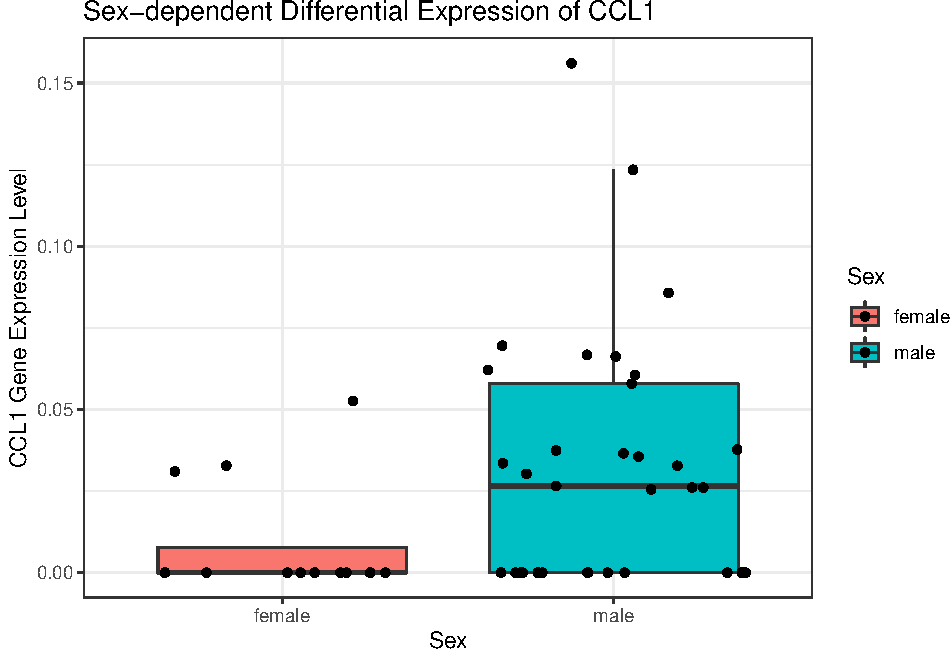
\includegraphics{LiuKevin_Final_Project_files/figure-latex/unnamed-chunk-17-1.pdf}

\begin{Shaded}
\begin{Highlighting}[]
\CommentTok{\# make box plot of BMP1 and OSMR gene expression levels between age groups faceted }
\CommentTok{\# by the gene}
\NormalTok{gene\_sample }\SpecialCharTok{\%\textgreater{}\%} 
  \CommentTok{\# keep only the columns we will use, otherwise pivot\_longer() doesn\textquotesingle{}t like it}
  \FunctionTok{select}\NormalTok{(BMP1, OSMR, age\_group) }\SpecialCharTok{\%\textgreater{}\%} 
  \FunctionTok{pivot\_longer}\NormalTok{(}\AttributeTok{cols =} \FunctionTok{c}\NormalTok{(BMP1, OSMR)) }\SpecialCharTok{\%\textgreater{}\%} \CommentTok{\# convert to long data format for faceted plots}
  \FunctionTok{filter}\NormalTok{(age\_group }\SpecialCharTok{!=} \StringTok{"Unknown"}\NormalTok{) }\SpecialCharTok{\%\textgreater{}\%} \CommentTok{\# filter out any samples with unknown age}
  \FunctionTok{ggplot}\NormalTok{(}\FunctionTok{aes}\NormalTok{(}\AttributeTok{x =}\NormalTok{ age\_group, }\AttributeTok{y =}\NormalTok{ value, }\AttributeTok{fill =}\NormalTok{ age\_group)) }\SpecialCharTok{+}
  \CommentTok{\# remove the outliers in this layer to avoid double{-}plotting}
  \FunctionTok{geom\_boxplot}\NormalTok{(}\AttributeTok{outlier.shape =} \ConstantTok{NA}\NormalTok{) }\SpecialCharTok{+} 
  \FunctionTok{geom\_jitter}\NormalTok{() }\SpecialCharTok{+} \CommentTok{\# add jittered data points on top of the box plots}
  \FunctionTok{facet\_wrap}\NormalTok{(}\SpecialCharTok{\textasciitilde{}}\NormalTok{name) }\SpecialCharTok{+} \CommentTok{\# facet by the gene names}
  \FunctionTok{labs}\NormalTok{(}\AttributeTok{x =} \StringTok{"Age Group"}\NormalTok{, }\AttributeTok{y =} \StringTok{"Gene Expression Level"}\NormalTok{, }\AttributeTok{fill =} \StringTok{"Age Group"}\NormalTok{, }
       \AttributeTok{title =} \StringTok{"Age{-}dependent Differential Expression of BMP1 and OSMR Genes"}\NormalTok{) }\SpecialCharTok{+}
  \FunctionTok{theme\_bw}\NormalTok{()}
\end{Highlighting}
\end{Shaded}

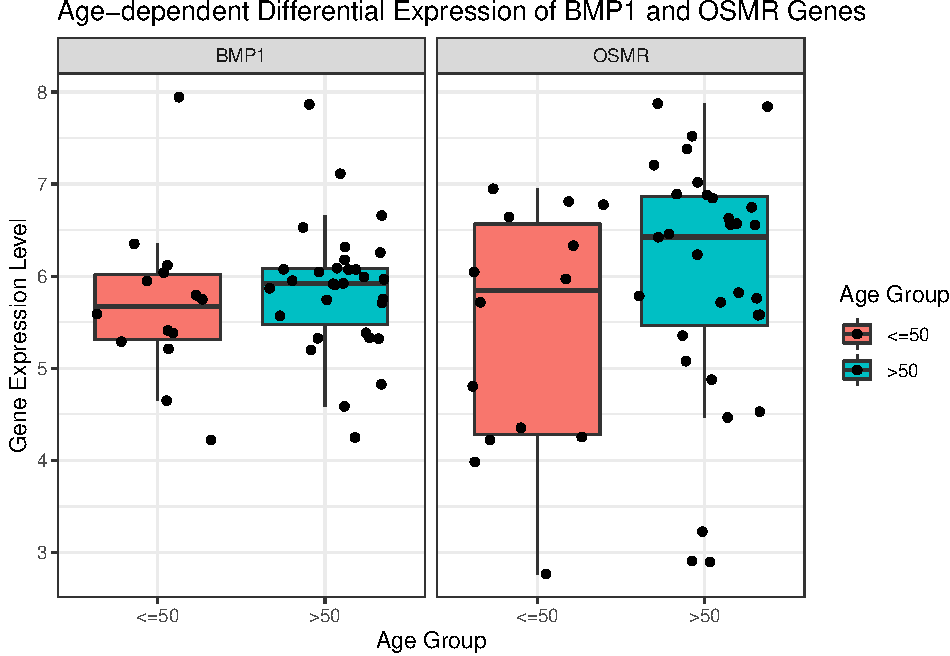
\includegraphics{LiuKevin_Final_Project_files/figure-latex/unnamed-chunk-17-2.pdf}

Based on the above plots, we have verified that males express higher
levels of CCL1 than females and both BMP1 and OSMR are expressed at
higher levels in those with ages greater than 50yo, supporting the
findings of Liang et al.

\end{document}
